\documentclass{article}

% ---------------------------------------------------------------------------
% Style file: prefer the REAL official ICLR 2027 style if it has been placed
% in this directory; otherwise fall back to a clearly-labeled placeholder
% (see iclr2027_fallback_shim.sty for why -- this sandbox has no general
% internet access and the real file could not be fetched or verified).
% No edits are needed here once the real .sty/.bst are added: just drop them
% into paper/ as iclr2027_conference.sty / iclr2027_conference.bst.
% ---------------------------------------------------------------------------
\usepackage{iftex}
\newif\ifhasrealstyle
\IfFileExists{iclr2027_conference.sty}{\hasrealstyletrue}{\hasrealstylefalse}
\ifhasrealstyle
  \usepackage{iclr2027_conference}
\else
  \usepackage{iclr2027_fallback_shim}
\fi

% \iclrfinalcopy is intentionally NEVER invoked -- double-blind stays on.

\usepackage[utf8]{inputenc}
\usepackage[T1]{fontenc}
\usepackage{amsmath,amssymb,amsfonts}
\usepackage{graphicx}
\usepackage{booktabs}
\usepackage{multirow}
\usepackage{xcolor}
\usepackage{pifont}
% Only the architecture diagram (figures/architecture.tex) is still live TikZ -- every other
% figure is a pre-rendered vector PDF (paper/figures/render_figures.py) placed via
% \includegraphics, specifically to keep Overleaf's per-pass compile time low (cleveref/
% hyperref/xr-hyper/natbib require 3-4 full recompiles, and re-executing PGFPlots from source
% on every one of those passes was the dominant cost). pgfplots/pgfplotstable/groupplots are
% therefore not loaded here at all.
\usepackage{tikz}
\usetikzlibrary{arrows.meta,positioning,shapes.geometric,fit,matrix,calc}
\usepackage{caption}
\usepackage{subcaption}
\usepackage{natbib}
\IfFileExists{iclr2027_conference.bst}{\bibliographystyle{iclr2027_conference}}{\bibliographystyle{plainnat}}

\usepackage[
  pdftitle={Domain-Aligned Compact Graph Diffusion for Zero-Shot Cross-City Severe-Congestion Classification},
  pdfauthor={},
  pdfsubject={},
  pdfkeywords={},
  pdfcreator={},
  pdfproducer={},
  colorlinks=true, linkcolor=blue, citecolor=blue, urlcolor=blue,
]{hyperref}

% cleveref must load after hyperref (and is conventionally loaded last of all packages).
\usepackage[capitalize,noabbrev]{cleveref}

\newcommand{\methodname}{ShiftGuard-RUGD}

\title{Domain-Aligned Compact Graph Diffusion for Zero-Shot \\ Cross-City Severe-Congestion Classification}
\author{Anonymous authors \\ Paper under double-blind review}
\date{}

\begin{document}
\maketitle

\ifhasrealstyle\else\PLACEHOLDERBANNER\fi

\begin{abstract}
% Every number in this abstract traces to outputs/studies/final_study/{main,ablations}/results_all.csv;
% see tables/headline.tex and tables/ablation.tex for the exact aggregation commands.
Traffic-congestion models are usually trained and evaluated on the same city, which hides a
practical failure mode: a newly instrumented city has no historical labels, and the operationally
important case -- rare, severe congestion -- is easy to miss while still scoring well on average.
We study zero-shot, source-only classification of severe congestion on an unseen city's road
network. We introduce \methodname{} (Robust Uncertainty-Guided Diffusion), a compact recurrent
graph classifier that couples an ID-free shared temporal/topological encoder with degree-normalized
graph diffusion, dual evidential supervision, effective-number rare-event weighting, and an
explicit gradient-reversal source-domain alignment term. Under a strictly leave-one-city-out,
chronologically embargoed protocol on the public OpenCity benchmark (three cities, three fixed
seeds, 99 main-suite and 63 matched-ablation runs, target labels touched only once at final
evaluation), a component-level ablation localizes the model's cross-city transfer almost entirely
to domain-adversarial alignment: removing it costs 3.44 severe-AUPRC points, roughly four times
the next-largest component effect (graph diffusion, 0.88 points) and roughly thirty times the
rare-event-specific mechanisms (class balancing, evidential supervision; $\le$0.11 points each).
Built around this mechanism, \methodname{} attains the best mean macro-F1 (0.8381$\pm$0.0112) and
severe-event AUPRC (0.8883$\pm$0.0310) among 11 compared models spanning non-learned, classical,
recurrent, and three clean-room Transformer/GNN adaptations, at 3--12$\times$ fewer parameters
(38K--67K) than the strongest competitor and with the best proper-scoring-rule calibration (NLL,
Brier) in the suite -- while its 95\% bootstrap interval over this margin overlaps the runner-up's,
and it is second, not first, under 30--50\% sensor dropout. We also trace an anomalous
uncertainty--error correlation in the two evidential models in the suite to a specific asymmetry in
the evidential KL regularizer that penalizes only target-class evidence, a diagnosis rather than a
fix. The evidence supports a compact, mechanistically localized, and honestly bounded operating
point for zero-shot severe-congestion classification, not a universal or state-of-the-art claim.
\end{abstract}


\section{Introduction}
\label{sec:intro}

Traffic-congestion forecasting is spatial, non-stationary, and operationally asymmetric: missing a
severe congestion event is not equivalent to a small error on free-flow speed. Most benchmarks
nevertheless train and evaluate on the same sensor network, optimize average regression error, and
report point predictions. Deploying to a newly instrumented city breaks every one of these
assumptions: the road topology changes, the sensor identities are new, the traffic regime differs,
and -- critically -- there are no historical labels for that city to train, calibrate, or select a
model against.

Prior work studies pieces of this problem separately. Traffic4Cast established spatial and temporal
transfer as a benchmark question \citep{eichenberger2022traffic4cast21,neun2022traffic4cast22};
CrossTReS, SFMGTL, and SCPT study cross-city or cross-road transfer, but typically fine-tune on
some target signal \citep{jin2022crosstres,chen2024sfmgtl,prabowo2024scpt}; STEP, UniST, and
OpenCity pursue pretrained or universal spatio-temporal prediction
\citep{shao2022step,yuan2024unist,li2025opencity}; and DeepSTUQ, UIGNN, STUP, and ensemble methods
address predictive uncertainty or missing observations, but within a fixed, previously-seen sensor
network \citep{qian2022deepstuq,mei2023uignn,jin2024stup,mallick2024ensemble,yu2025uqgnn}. None of
these lines jointly enforces target-label-free city transfer, a rare categorical endpoint, source-only
probabilistic calibration, and multiple controlled distribution shifts in one protocol -- a scoped
literature finding (\Cref{tab:literature-scope}), not a claim that no related paper exists anywhere.

This paper targets that joint setting with \methodname{} (Robust Uncertainty-Guided Diffusion), a
compact, ID-free recurrent graph classifier. Its architecture keeps the spatial mechanism
deliberately simple -- shared temporal encoding followed by degree-normalized diffusion and gated
residual fusion -- while local and final evidential heads, effective-number rare-event weighting,
and an explicit domain-adversarial alignment term shape the representation for transfer. The paper's
central empirical finding, established by a matched seven-variant ablation
(\Cref{sec:results,tab:ablation}), is that this transfer behavior is not distributed evenly across
the architecture: removing the domain-adversarial term costs roughly four times more severe-AUPRC
than removing graph diffusion, and roughly thirty times more than removing either rare-event
mechanism. We treat this as the paper's primary, falsifiable claim, and the model's competitive
standing among 11 baselines as a secondary consequence of building around that mechanism at a
compact scale -- rather than leading with the leaderboard position, whose 95\% bootstrap interval we
show overlaps the runner-up's (\Cref{sec:results}).

Our contributions are:
\begin{itemize}
  \item A chronological, embargoed, leave-one-city-out protocol in which target-city labels
        influence only the final, single evaluation pass -- with source-only thresholds,
        normalization, hyperparameter tuning, early stopping, and calibration, enforced in code and
        covered by a regression test (\Cref{sec:setup}).
  \item A compact, ID-free architecture integrating normalized graph diffusion, dual evidential
        supervision, effective-number rare-event weighting, and gradient-reversal source-domain
        alignment (\Cref{sec:method}), with an ablation that localizes cross-city transfer to a
        specific component rather than attributing it to the architecture as a whole.
  \item A comparison against ten baselines -- two non-learned sanity checks, three classical
        controls, two recurrent controls, and three clean-room adaptations of recent traffic
        Transformers/GNNs -- under matched splits, seeds, and (for four of the six tunable deep
        models) an equal Optuna tuning budget, with the tuning-budget asymmetry for the remaining
        two disclosed rather than hidden (\Cref{sec:setup}).
  \item Unusually broad, honestly reported evaluation: severe-event ranking metrics, calibration
        and conformal diagnostics, three families of controlled test-time corruption, efficiency,
        paired bootstrap and exact Wilcoxon inference with multiplicity correction, and a specific,
        code-level diagnosis of an anomalous uncertainty--error correlation in the two evidential
        models in the suite, rather than an unexplained residual (\Cref{sec:analysis}).
\end{itemize}

\section{Related Work}
\label{sec:related}

\paragraph{Spatiotemporal traffic models.} PDFormer models propagation delay and long-range
dependence \citep{jiang2023pdformer}; STAEformer shows that adaptive spatiotemporal embeddings make
a vanilla Transformer state-of-the-art \citep{liu2023staeformer}; TESTAM routes recurring and
non-recurring traffic through a mixture of experts \citep{lee2024testam}; and STID shows that simple
spatial/temporal identity embeddings are a strong, efficient baseline \citep{shao2022stid}, while
STEP augments graph forecasters with masked long-history pretraining \citep{shao2022step}. All
forecast continuous traffic variables within a fixed, previously-seen sensor network. Critically,
identity embeddings indexed by node or dataset -- central to STAEformer, STID, and most of this
family -- are not defined on a graph with an unseen node count; our ID-free encoder instead
conditions on shared history, calendar, and topology features that exist identically in any city.

\paragraph{Transfer and foundation models.} Traffic4Cast evaluates few-shot spatial transfer and
pandemic-era temporal shift \citep{eichenberger2022traffic4cast21,neun2022traffic4cast22}.
CrossTReS reweights source-city regions via domain adaptation and joint meta-learning, but its
protocol uses target data and fine-tuning \citep{jin2022crosstres}; SFMGTL uses semantic
multi-granularity transfer \citep{chen2024sfmgtl}; and SCPT learns representations for unseen roads
but assumes short target-road histories at inference \citep{prabowo2024scpt}. UniST combines
multi-scenario pretraining with knowledge-guided prompts \citep{yuan2024unist}; OpenCity pretrains
graph--Transformer blocks over heterogeneous traffic data for zero-shot forecasting
\citep{li2025opencity}. STONE studies joint structural/temporal out-of-distribution generalization
\citep{wang2024stone}, and a graphon-mixture approach targets cross-year spatial shift
\citep{wang2024spatialshift}. Our held-out city is excluded from training, label construction,
selection, and calibration, and the prediction target is rare-state classification, not continuous
regression -- a stricter and operationally different endpoint from any of the above.

\paragraph{Uncertainty and missing data.} DeepSTUQ unifies several uncertainty sources with
temperature-scaling calibration \citep{qian2022deepstuq}; UIGNN combines inductive prediction at
unobserved locations with uncertainty \citep{mei2023uignn}; STUP modulates propagation with
uncertainty \citep{jin2024stup}; scalable deep ensembles decompose uncertainty in graph forecasting
\citep{mallick2024ensemble}; and, most recently, UQGNN couples an interaction-aware spatiotemporal
embedding with a probabilistic prediction head evaluated on three in-network cities
\citep{yu2025uqgnn}. None of these evaluates uncertainty under leave-one-city-out transfer. Neither
evidential learning nor uncertainty-aware traffic modeling is claimed as new here; our contribution
is protocol-level -- source-only probabilistic calibration and conformal prediction sets evaluated
jointly with rare-event ranking and explicit test-time corruptions -- and, in \Cref{sec:analysis}, a
specific mechanistic diagnosis of where the evidential formulation's uncertainty quality breaks down.

\paragraph{Precise novelty boundary.} \methodname{} does not claim to invent recurrent encoding,
graph message passing, domain-adversarial training \citep{ganin2015dann}, Dirichlet evidential
heads \citep{sensoy2018evidential}, effective-number class weighting \citep{cui2019effectivenumber},
or conformal prediction \citep{angelopoulos2021gentle} in isolation. Its contribution is a specific
compact composition for a stricter operating point -- ID-free shared encoding permits unseen graph
sizes; degree normalization makes transport insensitive to city-specific node degree; local and
final evidential objectives supervise rare-class evidence before and after propagation; and
source-city adversarial training discourages source-specific representations -- combined with an
ablation that attributes the resulting transfer behavior to a specific one of these components
rather than to the composition as an undifferentiated whole. \Cref{app:literature-scope} tabulates
this scope claim directly against all 19 audited papers on six protocol dimensions (zero-shot
city transfer, rare/severe focus, predictive uncertainty, shift stress, conformal prediction,
efficiency focus); none combines more than two.

\section{Problem and Method}
\label{sec:method}

Let city $c$ have road graph $G_c=(V_c,A_c)$ and observed speeds $x^c_{t,i}$. Twelve half-hour bins
and their observation masks predict the next bin's class. For a held-out city $c^\star$, every
learned parameter and every fitted statistic (normalization, class thresholds, calibration) is
computed without access to $c^\star$'s labels. Normal, warning, and severe classes are separated by
the 30th and 10th percentiles of \emph{source-training} speed only.

\begin{figure}[t]
  \centering
  \resizebox{\linewidth}{!}{% Source: src/traffic_ml/opencity_models.py (DeepTrafficModel forward pass) and
% src/traffic_ml/losses.py (focal_evidential_loss, GradientReverse). Notation matches Method
% Eqs. 1-5 (alpha^loc, m_i, h_i, s_i, z_i, alpha_i) -- symbols are labeled on arrows here; full
% formulas live in the Method text rather than being repeated in the figure.
%
% Third revision, compacted: the 2nd revision's natural bounding box was ~26x20cm, which
% \resizebox{\linewidth}{!}{...} would have shrunk to an illegibly small font once scaled down
% to fit the page width (font size scales with the same factor as everything else). This
% version uses fixed absolute coordinates (as the 2nd revision did, to keep every box's
% position and gap checkable directly from source rather than only after a render) but with a
% tightened grid, bringing the natural footprint down to roughly 19x10.5cm -- scaling to
% \linewidth now shrinks text by a much smaller, still-legible factor. The in-figure legend
% (a further source of both height and of the exact nested-node-in-node pattern that caused a
% "TeX capacity exceeded" error in an earlier revision) is removed entirely; the color/style key
% is given in the caption instead, which is both safer and more compact.
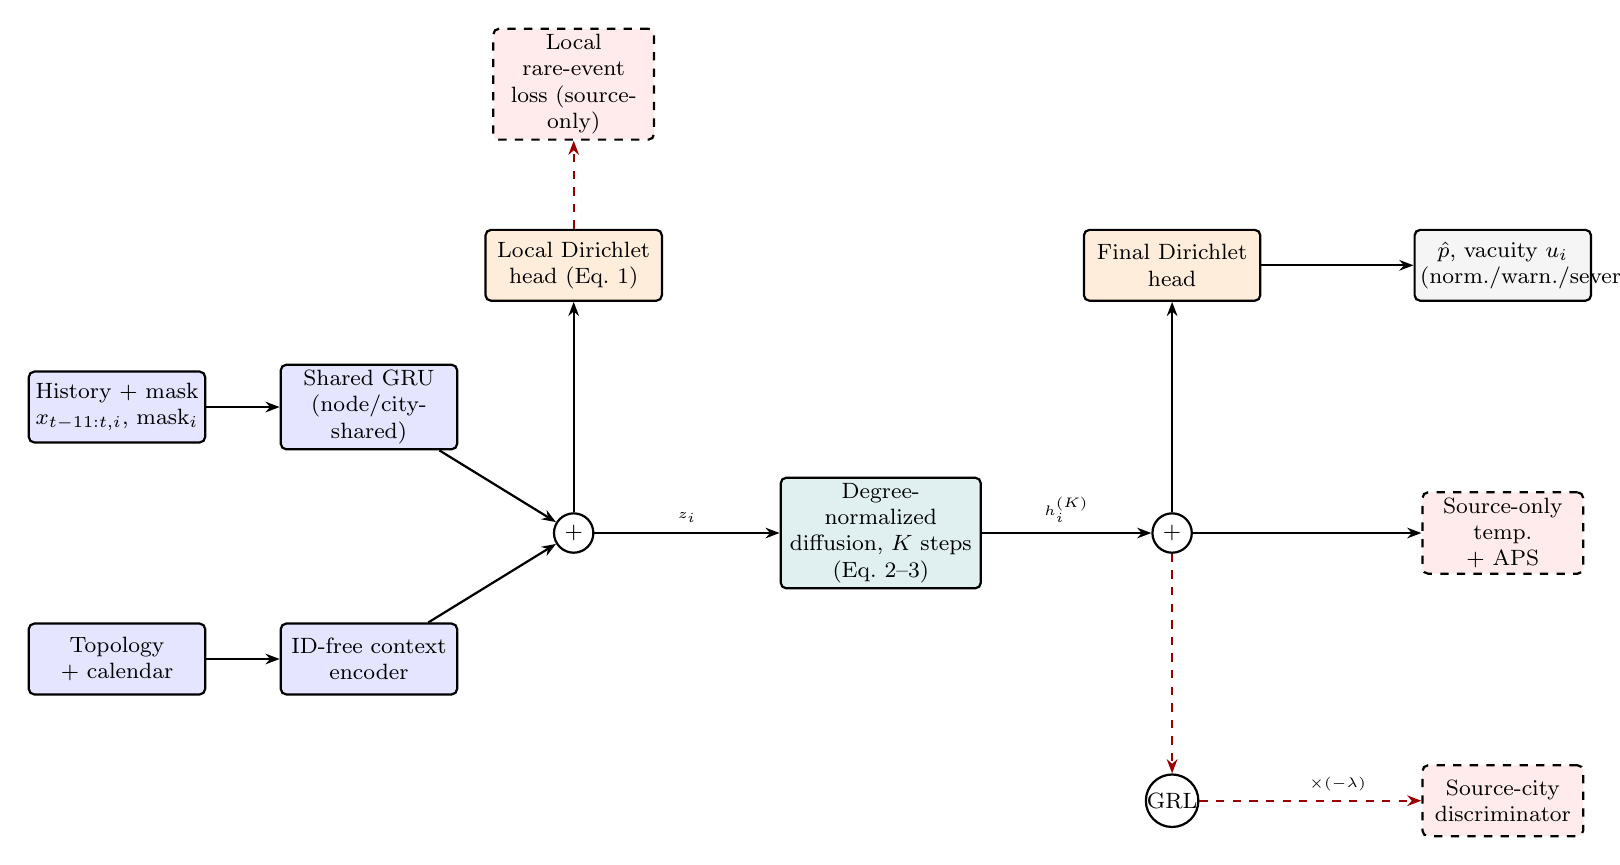
\begin{tikzpicture}[
  font=\footnotesize,
  >=Stealth,
  every node/.style={align=center},
  block/.style={draw, thick, rounded corners=2pt, minimum height=9mm, text width=21mm, fill=blockfill, inner sep=2pt},
  encoder/.style={block, fill=encfill},
  head/.style={block, fill=headfill},
  aux/.style={block, dashed, fill=auxfill, text width=19mm},
  diff/.style={block, fill=difffill, text width=24mm, minimum height=12mm},
  op/.style={circle, draw, thick, inner sep=0pt, minimum size=5mm, fill=white},
  train/.style={-{Stealth[length=1.8mm]}, dashed, thick, color=trainedge},
  infer/.style={-{Stealth[length=1.8mm]}, thick, color=inferedge},
  lbl/.style={font=\tiny, midway, above, sloped},
]

\colorlet{encfill}{blue!10}
\colorlet{headfill}{orange!14}
\colorlet{difffill}{teal!12}
\colorlet{auxfill}{red!8}
\colorlet{blockfill}{gray!8}
\colorlet{trainedge}{red!60!black}
\colorlet{inferedge}{black}

% ---- shared encoders ----
\node[encoder] (hist) at (0,1.6)    {History + mask\\ $x_{t-11:t,i}$, mask$_i$};
\node[encoder] (topo) at (0,-1.6)   {Topology + calendar};
\node[encoder] (gru)  at (3.2,1.6)  {Shared GRU\\ (node/city-shared)};
\node[encoder] (ctx)  at (3.2,-1.6) {ID-free context\\ encoder};

% ---- fusion 1 + local evidential branch ----
\node[op]   (fuse1)     at (5.8,0)    {$+$};
\node[head] (localhead) at (5.8,3.4)  {Local Dirichlet\\ head (Eq.~1)};
\node[aux]  (localloss) at (5.8,5.7)  {Local rare-event\\ loss (source-only)};

% ---- diffusion core ----
\node[diff] (diffusion) at (9.7,0) {Degree-normalized\\ diffusion, $K$ steps\\ (Eq.~2--3)};

% ---- fusion 2 + final head/output ----
\node[op]    (fuse2)     at (13.4,0)   {$+$};
\node[head]  (finalhead) at (13.4,3.4) {Final Dirichlet\\ head};
\node[block] (out)       at (17.6,3.4) {$\hat p$, vacuity $u_i$\\ (norm./warn./severe)};
\node[aux]   (calib)     at (17.6,0)   {Source-only temp.\\ + APS};

% ---- domain alignment (training-only) ----
\node[op]  (grl)  at (13.4,-3.4) {GRL};
\node[aux] (disc) at (17.6,-3.4) {Source-city\\ discriminator};

% ---- inference path (solid) ----
\draw[infer] (hist) -- (gru);
\draw[infer] (topo) -- (ctx);
\draw[infer] (gru) -- (fuse1);
\draw[infer] (ctx) -- (fuse1);
\draw[infer] (fuse1) -- (localhead);
\draw[infer] (fuse1) -- (diffusion) node[lbl] {$z_i$};
\draw[infer] (diffusion) -- (fuse2) node[lbl] {$h_i^{(K)}$};
\draw[infer] (fuse2) -- (finalhead);
\draw[infer] (finalhead) -- (out);
\draw[infer] (fuse2) -- (calib);
% No edge from localhead to out: per Method Sec. 3.1 the local evidential head does not alter
% spatial transport and has no forward path to the final output -- only the training-time
% auxiliary loss below (dashed).

% ---- training-only path (dashed) ----
\draw[train] (localhead) -- (localloss);
\draw[train] (fuse2) -- (grl);
\draw[train] (grl) -- (disc);
\node[font=\tiny] at ($(grl)!0.5!(disc)$) [above] {$\times(-\lambda)$};

\end{tikzpicture}
}
  \caption{\methodname{} architecture. Solid arrows: inference path. Dashed arrows: training-only
  (the local auxiliary loss and the gradient-reversal domain discriminator). Node fill keys the
  four component types: blue -- shared encoder, orange -- evidential (Dirichlet) head, teal --
  degree-normalized diffusion, red (dashed border) -- source-only auxiliary module. Notation
  matches \Cref{eq:local-evidential,eq:diffusion-message,eq:diffusion-update,eq:classification-loss,eq:total-loss}
  exactly. Redrawn as vector TikZ from the architecture implemented in
  \texttt{src/traffic\_ml/opencity\_models.py}; see \Cref{app:figure-redesign} for what changed
  from the earlier illustrative version and why.}
  \label{fig:architecture}
\end{figure}

\subsection{Shared encoding and normalized diffusion}
\label{sec:method-diffusion}

A single GRU, shared across every node and every city, encodes each node's normalized history and
observation mask into a temporal state $h_i$. An ID-free topology/calendar encoder produces static
context $s_i$ from four graph-derived static features (log in-/out-degree and their mean-normalized
versions, computed from the adjacency matrix itself) and four calendar features (sine/cosine of
time-of-day and day-of-week) -- available identically in any city, unlike a learned per-node or
per-city embedding. Their fusion $z_i$ feeds a local evidential head,
\begin{equation}
  \boldsymbol\alpha_i^{\mathrm{loc}} = \mathrm{softplus}(W_{\mathrm{loc}} z_i) + \mathbf{1}, \qquad
  u_i^{\mathrm{loc}} = K \big/ \textstyle\sum_k \alpha_{ik}^{\mathrm{loc}},
  \label{eq:local-evidential}
\end{equation}
with $K=3$. The local head receives source supervision (\Cref{eq:classification-loss}) but does not
alter spatial transport. Each of $K_{\mathrm{diff}}$ diffusion layers computes a degree-normalized
message and a gated residual update,
\begin{align}
  m_i^{(\ell)} &= \frac{\sum_j A_{ij} h_j^{(\ell)}}{\max\!\big(\sum_j A_{ij},\ \epsilon\big)},
  \label{eq:diffusion-message} \\
  h_i^{(\ell+1)} &= \mathrm{LN}\Big(h_i^{(\ell)} + \sigma\big(W_g[h_i^{(\ell)}; m_i^{(\ell)}; 1]\big)
  \odot \tanh\big(W_m[h_i^{(\ell)}; m_i^{(\ell)}]\big)\Big).
  \label{eq:diffusion-update}
\end{align}
The constant context term in the gate retains a checkpoint-compatible residual parameterization
across ablation variants. $K_{\mathrm{diff}}=2$ in the final tuned configuration
(\Cref{app:hyperparameters}). Final fusion of $h_i^{(K_{\mathrm{diff}})}$ with $s_i$ produces the
final Dirichlet parameters $\boldsymbol\alpha_i=\mathrm{softplus}(W_o h_i)+\mathbf{1}$, expected
class probabilities $\hat p_i = \alpha_i/\sum_k \alpha_{ik}$, and vacuity $u_i=K/\sum_k\alpha_{ik}$.

\subsection{Rare-event and domain objectives}
\label{sec:method-loss}

Effective-number weights \citep{cui2019effectivenumber} counter class imbalance, and focal
modulation (exponent $\gamma$, tuned per run; \Cref{app:hyperparameters}) emphasizes hard examples.
Writing
$S_i=\sum_k\alpha_{ik}$, $p_{ik}=\alpha_{ik}/S_i$, and $y_i$ for the target class, the final
classification term is
\begin{equation}
  \mathcal{L}_{\mathrm{cls}} = -w_{y_i}(1-p_{i,y_i})^\gamma \log p_{i,y_i}
    + \lambda_{\mathrm{KL}}\, \mathrm{KL}\!\big[\mathrm{Dir}(\tilde{\boldsymbol\alpha}_i)
    \,\|\, \mathrm{Dir}(\mathbf{1})\big],
  \label{eq:classification-loss}
\end{equation}
where $w_k \propto (1-\beta)/(1-\beta^{n_k})$ is normalized across classes
\citep{cui2019effectivenumber}, and $\tilde{\boldsymbol\alpha}_i$ retains the predicted
\emph{true-class} concentration $\alpha_{i,y_i}$ while setting every non-target concentration to
one before the KL penalty is computed (\texttt{src/traffic\_ml/losses.py::focal\_evidential\_loss},
lines 31--33). We flag this construction explicitly here rather than leave it implicit: the
standard evidential-deep-learning KL regularizer \citep{sensoy2018evidential} penalizes evidence
accumulated on \emph{incorrect} classes, to suppress overconfident wrong predictions; the
construction above penalizes evidence only on the \emph{correct} class. \Cref{sec:analysis} traces
this asymmetry to an observed downstream effect and argues it is the most likely explanation for it.
The identical construction (minus the domain term) defines the local auxiliary loss, weighted
$\lambda_{\mathrm{loc}}$ against the final loss.

A gradient-reversal layer \citep{ganin2015dann} -- identity in the forward pass, its gradient
scaled by $-\lambda_{\mathrm{dom}}(t)$ in the backward pass, with $\lambda_{\mathrm{dom}}(t)$ ramped
by a sigmoid schedule from 0 to 1 over training -- feeds the mean-pooled final representation into a
small MLP trained to predict which \emph{source} city produced the sample. Because the gradient is
reversed, the encoder is trained to make its representation \emph{indistinguishable} across source
cities, which is the mechanism this paper argues (\Cref{sec:results}, ablations) is primarily
responsible for the transfer behavior to a third, unseen city. The total loss is
\begin{equation}
  \mathcal{L} = \mathcal{L}_{\mathrm{final}} + \lambda_{\mathrm{loc}}\,\mathcal{L}_{\mathrm{local}}
  + \lambda_{\mathrm{dom}}\,\mathcal{L}_{\mathrm{domain}}.
  \label{eq:total-loss}
\end{equation}
No node or city identity embedding is available to the predictor at any point in this pipeline.
Temperature scaling and adaptive prediction-set (APS) conformal calibration
\citep{angelopoulos2021gentle} are fitted only on chronological source calibration segments,
following split-conformal practice; because exchangeability between source calibration cities and
an unseen target city is not guaranteed by construction, we report APS coverage on the target
diagnostically (\Cref{sec:results}) rather than as a formal target-city guarantee.

\section{Experimental Setup}
\label{sec:setup}

\paragraph{Data and splits.} We use the OpenCity-packaged TrafficCD, TrafficHZ, and TrafficSH
road-sensor graphs \citep{neun2022traffic4cast22,li2025opencity}: 1{,}403 half-hour bins over
728, 672, and 896 nodes respectively. In every leave-one-city-out fold, the two source cities are
partitioned chronologically into 65\% train, 10\% calibration, and 10\% validation, separated by a
12-bin (6-hour) embargo; the held-out city contributes only its final chronological 15\% segment,
evaluated once, after every decision is frozen. Source-only severe/warning thresholds for the
TrafficCD/HZ/SH folds are 6.2648/7.7861, 6.4688/7.9714, and 6.0548/7.4192
(\texttt{outputs/studies/final\_study/main/*/rugd/seed\_*/target\_definition.json}).

\paragraph{Baselines.} Non-learned sanity checks are the source class-frequency prior and
last-observation persistence. Classical controls are balanced logistic regression, histogram
gradient boosting, and LightGBM, each run with fixed, standard hyperparameters (\texttt{C=1},
\texttt{max\_iter=250}/\texttt{500}, \texttt{num\_leaves=63}, class-balanced weighting;
\texttt{src/traffic\_ml/opencity\_classical.py}) rather than an Optuna search -- we state this
explicitly rather than imply parity with the tuned neural models, since these are included as
strong non-neural reference points, not as tuning-matched competitors. Neural controls are GRU and
Graph-GRU. We also implement inductive task adaptations of STAEformer \citep{liu2023staeformer},
UIGNN \citep{mei2023uignn}, and OpenCity \citep{li2025opencity}: adaptations preserve each paper's
defining mechanism but replace a fixed-graph regression head with a shared node-wise classification
head. The UIGNN adaptation retains bidirectional Chebyshev diffusion and recovery regularization;
STAEformer retains temporal patching, adaptive spatiotemporal embeddings, and self-attention (with
its dataset-indexed node embeddings replaced by our topology-conditioned features, since the
originals are undefined on an unseen graph); OpenCity-Scratch retains masked temporal modeling and
graph-aware Transformer blocks. All models receive identical histories, source-only thresholds,
splits, output classes, and evaluation code, and none is claimed as an official reproduction.
Released OpenCity checkpoints are excluded because their public pretraining set includes TrafficCD
and TrafficHZ, which would contaminate zero-shot evaluation on those cities.

\paragraph{Tuning budget (disclosed asymmetry).} RUGD, UIGNN, and the two Transformer adaptations
were tuned with source-only Optuna search under an identical objective (below); this is directly
evidenced in this study's run logs (12 completed searches: RUGD and UIGNN at 20 trials/city, the
two Transformers at 8 compute-matched trials/city). \textbf{GRU and Graph-GRU were not tuned within
this study's logged pipeline}: their final configurations were carried in as fixed,
RUGD-search-space-matched hyperparameters from an earlier tuning pass whose trial records are not
part of this study's retained artifacts. We report this as a limitation on tuning parity for these
two specific baselines rather than omit it (\Cref{sec:limitations}); the four models that were
tuned within this study (RUGD, UIGNN, STAEformer-Inductive, OpenCity-Scratch) remain fully
evidenced and mutually parity-comparable. The shared objective weights clean macro-F1 (0.40),
clean severe AUPRC (0.30), and 30\%-missing macro-F1/AUPRC (0.15 each), computed per source city
and averaged so the larger source graph does not dominate selection; the exact formula and full
per-hyperparameter search ranges are in \Cref{app:hyperparameters}. Target labels never enter
tuning, selection, or calibration at any stage (enforced in code and covered by a regression
test; \Cref{sec:limitations}).

\paragraph{Seeds and runs.} Three fixed seeds (17, 42, 2025) $\times$ 3 held-out cities $\times$
11 models = 99 main-suite runs, plus 3 cities $\times$ 7 RUGD-variant ablations $\times$ 3 seeds =
63 matched ablation runs -- 162 registered training runs total, each with a checkpoint,
predictions, and a \texttt{provenance.json} recording the exact resolved configuration. No seed or
run is omitted from any reported aggregate.

\paragraph{Evaluation.} Primary metrics are macro-F1 and severe-class AUPRC. Secondary metrics
include severe precision/recall/F1/AUROC, balanced accuracy, NLL, Brier score, ECE, ACE,
uncertainty--error Spearman correlation, APS coverage/set size, parameter count, training time, and
inference throughput. Stress tests independently mask 10/30/50\% of observations, add Gaussian
noise at $\sigma\in\{0.1,0.3\}$, or roll input histories by one or two bins, in each case reusing
clean-fit source calibration (not re-tuned per condition) to measure generalization robustness
rather than re-calibrated robustness. Paired inference on timestamp-level NLL differences uses
block bootstrap and Wilcoxon tests; the headline 30\%/50\%-missing AUPRC comparisons use the nine
paired city--seed scores, exact two-sided Wilcoxon tests, rank-biserial effect sizes, a 20{,}000-draw
hierarchical city-then-seed bootstrap, and Holm correction across learned baselines. Because three
seeds on one city are not three independent geographies, we additionally report an exact sign-flip
test over the three city-level means as a conservative sensitivity check; its minimum achievable
two-sided $p$-value with three cities is 0.25, so no city-level/geographic significance is claimed
anywhere in this paper.

\section{Results}
\label{sec:results}

\subsection{Clean zero-shot performance}
\label{sec:results-clean}

% Source: outputs/studies/final_study/main/results_all.csv (mean/SD) and
% outputs/studies/final_study/main/headline_bootstrap_ci.csv (95% CI, 20,000-repeat
% hierarchical city-then-seed bootstrap -- the SAME construction as every paired-
% comparison CI in this paper; see paper/tables/regenerate_headline_ci.py).
% Regenerate with: python paper/tables/generate_tables.py
\begin{table}[t]
\centering
\caption{Held-out-city results, mean $\pm$ sample SD over nine city--seed runs (3 cities $\times$ 3 seeds), with 95\% bootstrap confidence intervals on the two primary metrics. Bold marks the best mean per column. Note the RUGD/STAEformer intervals overlap on both primary metrics (\Cref{sec:results}).}
\label{tab:headline}
\resizebox{\linewidth}{!}{%
\begin{tabular}{lccccc}
\toprule
Method & Macro-F1 $\uparrow$ & 95\% CI & Severe AUPRC $\uparrow$ & 95\% CI & NLL $\downarrow$ \\
\midrule
\textbf{ShiftGuard-RUGD} & \textbf{0.8381}$\pm$0.0112 & [0.8271, 0.8523] & \textbf{0.8883}$\pm$0.0310 & [0.8589, 0.9281] & \textbf{0.2625}$\pm$0.0427 \\
STAEformer-Inductive & 0.8302$\pm$0.0138 & [0.8137, 0.8427] & 0.8815$\pm$0.0368 & [0.8418, 0.9257] & 0.2681$\pm$0.0455 \\
Graph-GRU & 0.8298$\pm$0.0086 & [0.8225, 0.8391] & 0.8785$\pm$0.0276 & [0.8556, 0.9116] & 0.2789$\pm$0.0574 \\
GRU & 0.8282$\pm$0.0132 & [0.8137, 0.8430] & 0.8799$\pm$0.0330 & [0.8475, 0.9199] & 0.2735$\pm$0.0473 \\
OpenCity-Scratch & 0.8280$\pm$0.0135 & [0.8133, 0.8415] & 0.8770$\pm$0.0338 & [0.8408, 0.9180] & 0.2770$\pm$0.0493 \\
LightGBM & 0.8210$\pm$0.0119 & [0.8064, 0.8333] & 0.8775$\pm$0.0343 & [0.8426, 0.9204] & 0.3008$\pm$0.0541 \\
HGBDT & 0.8192$\pm$0.0123 & [0.8044, 0.8319] & 0.8765$\pm$0.0348 & [0.8409, 0.9201] & 0.3066$\pm$0.0546 \\
Persistence & 0.8186$\pm$0.0137 & [0.8040, 0.8353] & 0.6270$\pm$0.0685 & [0.5654, 0.7162] & 0.4519$\pm$0.0553 \\
UIGNN-Inductive & 0.8179$\pm$0.0136 & [0.8044, 0.8341] & 0.8568$\pm$0.0395 & [0.8218, 0.9077] & 0.2991$\pm$0.0511 \\
Logistic & 0.7841$\pm$0.0092 & [0.7721, 0.7915] & 0.7972$\pm$0.0507 & [0.7451, 0.8603] & 0.4328$\pm$0.0695 \\
Prior & 0.2642$\pm$0.0283 & [0.2268, 0.2872] & 0.1117$\pm$0.0505 & [0.0737, 0.1788] & 0.8494$\pm$0.1648 \\
\bottomrule
\end{tabular}}
\end{table}


\methodname{} leads the complete 11-model suite on both primary metrics
(\Cref{tab:headline}): macro-F1 0.8381$\pm$0.0112, 0.79 points above STAEformer-Inductive, and
severe AUPRC 0.8883$\pm$0.0310, 0.68 points above it. It also has the best mean NLL. \textbf{The
95\% hierarchical city-then-seed bootstrap intervals on both primary metrics overlap
STAEformer-Inductive's} -- macro-F1 [0.8271, 0.8523] vs.\ [0.8137, 0.8427]; severe AUPRC
[0.8589, 0.9281] vs.\ [0.8418, 0.9257] -- so we
present the leaderboard position as a real but not dominant point estimate, not as a
statistically separated win in isolation; \Cref{sec:ablations} gives the more specific,
mechanism-level claim this paper leads with. \Cref{fig:main-auprc} shows the full ranking.

\begin{figure}[t]
\centering
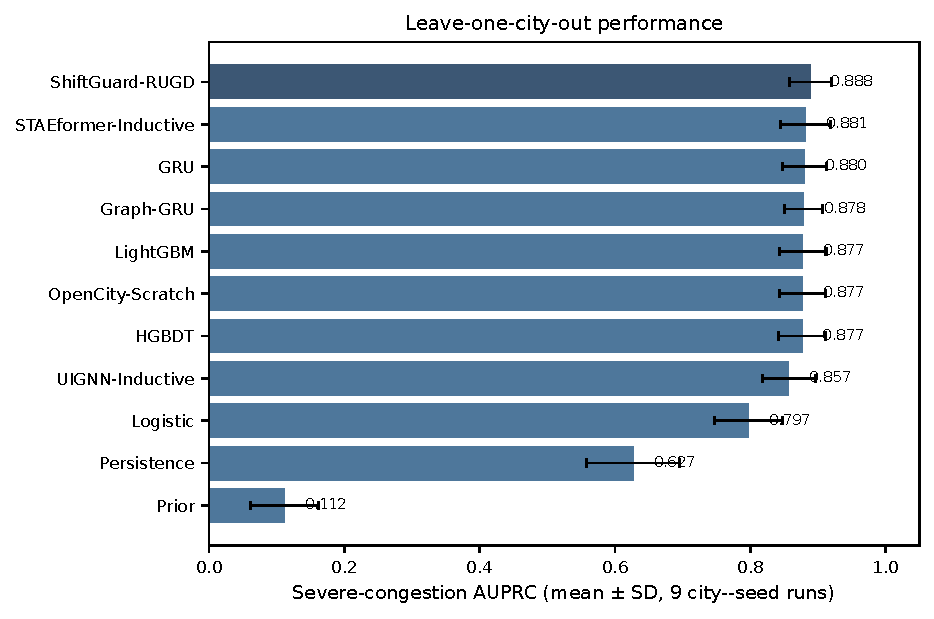
\includegraphics[width=0.85\linewidth]{figures/main_severe_auprc.pdf}
\caption{Severe-congestion AUPRC across all 11 compared models, mean $\pm$ SD over nine
city--seed runs. Source: \texttt{outputs/studies/final\_study/main/results\_all.csv}; rendered by
\texttt{paper/figures/render\_figures.py} from \texttt{paper/figures/data/main\_severe\_auprc.csv}.}
\label{fig:main-auprc}
\end{figure}

\subsection{Robustness under distribution shift}
\label{sec:results-robustness}

% Source: outputs/studies/final_study/main/robustness_all.csv, missingness rows only
% (full 7-condition table is tables/full_robustness.tex in the appendix).
% Regenerate with: python paper/tables/generate_tables.py
\begin{table}[t]
\centering
\caption{Severe AUPRC under 30\% and 50\% independently-masked sensor observations, mean $\pm$ SD over nine city--seed runs; clean-fit source calibration is reused (not re-tuned per condition). Bold marks the best mean per column. See \Cref{app:robustness-full} for all seven registered corruption conditions.}
\label{tab:robustness}
\resizebox{\linewidth}{!}{%
\begin{tabular}{lcc}
\toprule
Method & 30\% missing & 50\% missing \\
\midrule
\textbf{ShiftGuard-RUGD} & 0.7938$\pm$0.0532 & 0.7242$\pm$0.0718 \\
STAEformer-Inductive & \textbf{0.8139$\pm$0.0630} & \textbf{0.7459$\pm$0.0878} \\
Graph-GRU & 0.7408$\pm$0.0953 & 0.5421$\pm$0.2060 \\
GRU & 0.6900$\pm$0.0806 & 0.4734$\pm$0.1359 \\
OpenCity-Scratch & 0.6461$\pm$0.1285 & 0.3784$\pm$0.1885 \\
LightGBM & 0.5597$\pm$0.1253 & 0.3551$\pm$0.1289 \\
HGBDT & 0.5470$\pm$0.1345 & 0.3447$\pm$0.1334 \\
Persistence & 0.4750$\pm$0.0659 & 0.3703$\pm$0.0610 \\
UIGNN-Inductive & 0.7395$\pm$0.0509 & 0.6247$\pm$0.0597 \\
Logistic & 0.3164$\pm$0.0612 & 0.2192$\pm$0.0538 \\
Prior & 0.1117$\pm$0.0505 & 0.1117$\pm$0.0505 \\
\bottomrule
\end{tabular}}
\end{table}


Missing sensors expose \methodname{}'s clearest limitation: STAEformer-Inductive ranks first at
both 30\% and 50\% masking (\Cref{tab:robustness}), while \methodname{} is second, exceeding every
other learned baseline by a wide margin (e.g., +5.30 and +18.20 points over Graph-GRU at 30\%/50\%).
Under strong measurement noise and temporal shift, rankings are closer and no method dominates
every metric (\Cref{fig:robustness}; full seven-condition table in \Cref{app:robustness-full}).

\begin{figure}[t]
\centering
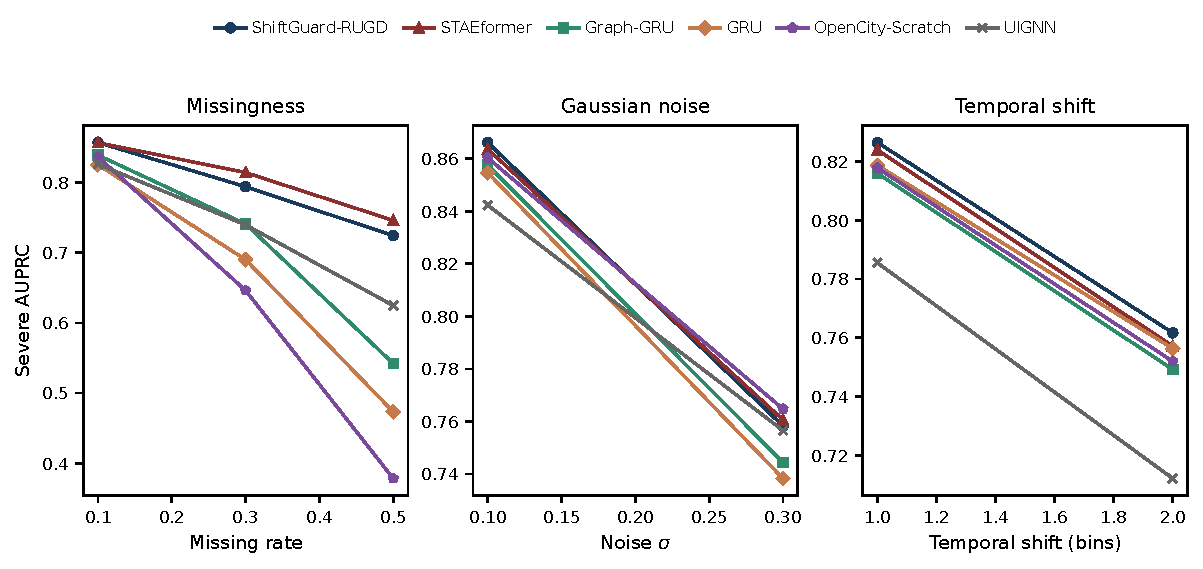
\includegraphics[width=\linewidth]{figures/robustness.pdf}
\caption{Severe AUPRC across all registered corruption severities for a six-model focus set.
Source: \texttt{outputs/studies/final\_study/main/robustness\_all.csv}; rendered by
\texttt{paper/figures/render\_figures.py}.}
\label{fig:robustness}
\end{figure}

\subsection{Component ablations localize the transfer mechanism}
\label{sec:ablations}

% Source: outputs/studies/final_study/ablations/results_all.csv, aggregated per
% variant over nine city-seed runs each.
% Regenerate with: python paper/tables/generate_tables.py
\begin{table}[t]
\centering
\caption{Final-architecture ablations, mean $\pm$ SD over nine city--seed runs each. $\Delta$ is clean severe-AUPRC change from full \methodname{}; bold marks the single largest-magnitude $\Delta$. Domain alignment's removal costs roughly $4\times$ the next-largest component effect (graph diffusion) and roughly $30\times$ the rare-event-specific mechanisms (class balance, evidence).}
\label{tab:ablation}
\begin{tabular}{lccccc}
\toprule
Variant removed & Macro-F1 & Clean severe AUPRC & $\Delta$ & NLL & ECE \\
\midrule
w/o graph diffusion & 0.8325$\pm$0.0128 & 0.8795$\pm$0.0336 & -0.0088 & 0.2714 & 0.0076 \\
w/o topology & 0.8308$\pm$0.0134 & 0.8786$\pm$0.0352 & -0.0097 & 0.2730 & 0.0079 \\
w/o domain alignment & 0.8221$\pm$0.0129 & 0.8538$\pm$0.0403 & \textbf{-0.0344} & 0.3024 & 0.0128 \\
w/o evidence & 0.8357$\pm$0.0113 & 0.8874$\pm$0.0314 & -0.0009 & 0.2632 & 0.0067 \\
w/o focal modulation & 0.8374$\pm$0.0117 & 0.8842$\pm$0.0288 & -0.0041 & 0.2698 & 0.0098 \\
w/o class balance & 0.8367$\pm$0.0116 & 0.8872$\pm$0.0320 & -0.0011 & 0.2626 & 0.0061 \\
\midrule
\textbf{Full ShiftGuard-RUGD} & \textbf{0.8381}$\pm$0.0112 & \textbf{0.8883}$\pm$0.0310 & --- & 0.2625 & 0.0066 \\
\bottomrule
\end{tabular}
\end{table}


\Cref{tab:ablation} and \Cref{fig:ablation-waterfall} give this paper's central, falsifiable
claim: removing domain-adversarial source alignment costs 3.44 severe-AUPRC points -- roughly
$4\times$ the next-largest component effect (graph diffusion, 0.88 points; transferable topology,
0.97 points) and roughly $30\times$ the two rare-event-specific mechanisms (class balancing,
$-0.11$ points; evidential supervision, $-0.09$ points, both within noise of zero). This is not
distributed credit across the architecture: the mechanism doing the heavy lifting for zero-shot
transfer specifically is the explicit cross-city domain-invariance pressure, not the spatial
diffusion or the rare-event machinery, both of which matter far more modestly. Class-balance and
evidential-head removals are, on this three-city sample, negative results -- essentially
noise-level -- and we report them as such rather than retrofit a story where every component
contributes comparably.

\begin{figure}[t]
\centering
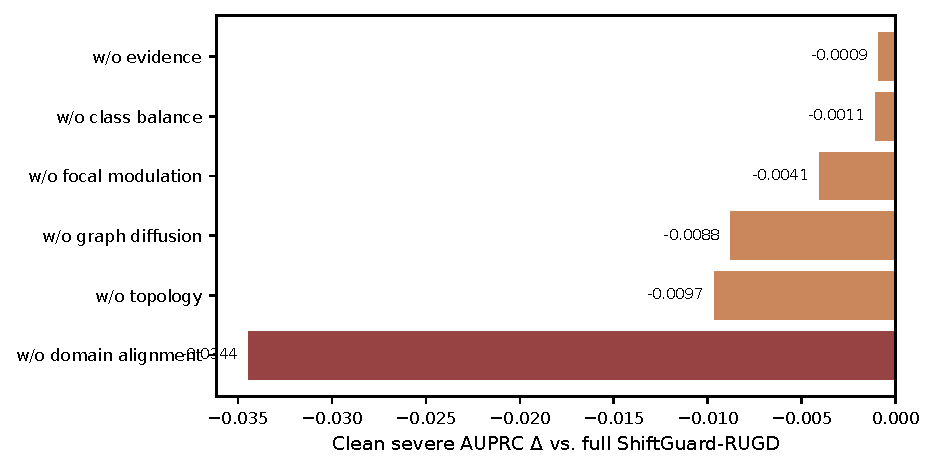
\includegraphics[width=0.85\linewidth]{figures/ablation_waterfall.pdf}
\caption{Clean severe-AUPRC change from removing each component, full \methodname{} as the
reference. Domain alignment dominates. Source:
\texttt{outputs/studies/final\_study/ablations/results\_all.csv}; rendered by
\texttt{paper/figures/render\_figures.py}.}
\label{fig:ablation-waterfall}
\end{figure}

\subsection{Per-city results}
\label{sec:results-percity}

TrafficHZ is the strongest case for \methodname{} (\Cref{tab:percity} in \Cref{app:percity-detail}:
0.8524 macro-F1, 0.9281 severe AUPRC). TrafficCD is a near-tie with STAEformer-Inductive and should
not be presented as a
decisive city-level result; TrafficSH shows a larger clean advantage over the attention-based
adaptations but the lowest absolute severe AUPRC of the three cities.

\subsection{Calibration and efficiency}
\label{sec:results-calib-eff}

\methodname{} has the best NLL and Brier score in the suite but not the best ECE (STAEformer is
lower); full calibration and parameter/throughput tables are in \Cref{app:calibration,app:efficiency}.
APS conformal coverage is 0.9984$\pm$0.0003 against a nominal 0.90 target with mean set size
2.1552$\pm$0.0834 -- substantially over-conservative, and, because source-calibration and an unseen
target city are not guaranteed exchangeable, we report this as an observed transfer result rather
than a formal coverage guarantee. \methodname{} is the smallest neural model in the suite
(38{,}048--66{,}600 parameters, 3--12$\times$ fewer than STAEformer-Inductive) and runs inference
roughly 3.5$\times$ faster than it, while training roughly 2$\times$ faster; it is slower to train
than the plain recurrent controls, since the diffusion, gating, and domain-adversarial machinery is
not free (\Cref{app:efficiency}). The confusion matrix and severe-event calibration/PR curves for
one registered run are given in \Cref{app:qualitative}: errors concentrate between adjacent
severity classes, consistent with the ordinal structure of the label space.

\section{Analysis: An Asymmetry in the Evidential KL Term}
\label{sec:analysis}

Every softmax-based model in the suite shows predicted uncertainty tracking prediction error at a
consistent Spearman $\rho\approx0.39$--$0.42$ (GRU 0.4014$\pm$0.0074, Graph-GRU 0.3868$\pm$0.0092,
STAEformer-Inductive 0.4019$\pm$0.0037, OpenCity-Scratch 0.3993$\pm$0.0062, and the three classical
controls at 0.42--0.43) -- exactly what a useful uncertainty estimate should do.
\textbf{The two Dirichlet/evidential models in the suite are the only outliers}: \methodname{} is
$-0.0526\pm0.0782$ and UIGNN-Inductive is $0.0061\pm0.0410$
(\texttt{outputs/studies/final\_study/main/results\_all.csv},
column \texttt{uncertainty\_error\_spearman}). Both anomalous models share the same evidential-KL
construction described in \Cref{eq:classification-loss}: the regularizer
$\mathrm{KL}[\mathrm{Dir}(\tilde{\boldsymbol\alpha}_i)\,\|\,\mathrm{Dir}(\mathbf{1})]$ is computed
on $\tilde{\boldsymbol\alpha}_i$, which retains the network's predicted concentration only at the
\emph{true} class index and fixes every other class's concentration to one
(\texttt{src/traffic\_ml/losses.py}, lines 31--33). Concretely, for a 3-class Dirichlet with
predicted concentrations $(\alpha_1,\alpha_2,\alpha_3)$ and true class $y=1$, the KL term sees
$\tilde{\boldsymbol\alpha}=(\alpha_1,1,1)$: whatever evidence the network accumulates on classes 2
and 3 is invisible to this regularizer regardless of whether the prediction was correct.

This is the reverse of the construction in \citet{sensoy2018evidential}, where the KL-to-uniform
penalty is applied to the concentrations \emph{excluding} the true class, specifically to suppress
unwarranted evidence on incorrect classes -- the mechanism by which evidential deep learning
produces uncertainty that grows with the plausibility of competing wrong answers. Under the
construction implemented here, a network can accumulate large, unpenalized evidence on an incorrect
class without any corresponding regularization pressure, which would manifest exactly as we observe
it: predicted vacuity that fails to track actual error, because the model's confidence is shaped by
a term that never sees where the network's evidence is misallocated.

We did not fix and re-run this construction: this sandboxed evaluation environment has no GPU and
no PyTorch installation, so a corrected KL term (regularizing non-target concentrations, matching
\citet{sensoy2018evidential}) could not be trained and evaluated end-to-end for this paper. We
report this as a specific, checkable diagnosis rather than a closed, fixed result, and we note two
things it does \emph{not} undermine: first, the headline accuracy numbers in
\Cref{sec:results-clean} come from $\arg\max$ over the Dirichlet expectation $\hat p_i=\alpha_i/\sum_k
\alpha_{ik}$, not from the KL term directly, so this asymmetry does not implicate the classification
results; second, it is consistent, specific, and falsifiable -- a corrected implementation predicts
both anomalous models' uncertainty--error correlation should move toward the $\rho\approx0.4$ band
shared by every softmax baseline, which is a concrete, testable prediction for follow-up work rather
than an unexplained residual.

\section{Limitations}
\label{sec:limitations}

\textbf{Development status.} The final architecture was selected after inspecting all three
OpenCity folds during development; TrafficSH in particular was used in an earlier smoke study
(\texttt{rugd\_smoke\_v1}) that directly informed the normalized-diffusion design
(\texttt{docs/OPENCITY\_PROTOCOL.md}). All three folds are reported, but TrafficCD and TrafficHZ
are the primary confirmatory folds; TrafficSH is development evidence reported as a third fold,
not an untouched held-out geography. Target-city \emph{labels} never enter tuning or selection at
any stage (enforced in code and tested directly by
\texttt{tests/test\_opencity.py::test\_source\_statistics\_do\_not\_consult\_target}, which mutates
target-city data after fitting source statistics and asserts the fit is unchanged), but the
architecture itself was chosen with all three folds' unlabeled structure visible during
development. A genuinely unseen fourth city or an external dataset is the only way to settle
whether this design choice generalizes beyond three-city internal evidence.

\textbf{Tuning-budget asymmetry for two baselines.} As disclosed in \Cref{sec:setup}, GRU and
Graph-GRU were not tuned within this study's logged Optuna pipeline; their hyperparameters were
carried in from an earlier, unretained tuning pass. The four models that were tuned within this
study (RUGD, UIGNN-Inductive, STAEformer-Inductive, OpenCity-Scratch) remain fully evidenced and
mutually comparable; GRU/Graph-GRU's standing relative to those four should be read with this
asymmetry in mind.

\textbf{Not universally dominant.} STAEformer-Inductive wins under the two heaviest sensor-dropout
conditions (\Cref{tab:robustness}); \methodname{} is not robust to every registered condition, and
we do not claim it is. Attention over the full temporal window plausibly lets STAEformer recover
missing recent readings more gracefully than \methodname{}'s local temporal encoder plus
degree-normalized diffusion, but this mechanism has not been isolated experimentally -- a wider-
temporal-receptive-field variant of \methodname{} would be the natural follow-up ablation.

\textbf{No city-level statistical significance.} With three held-out cities, the exact sign-flip
test's minimum achievable two-sided $p$-value is 0.25 (\Cref{sec:setup}); no claim of geographic
generalization beyond these three cities is made anywhere in this paper. The paired, seed-level
Wilcoxon results (\Cref{app:paired-inference}) are strong (rank-biserial $=1.0$ against GRU,
Graph-GRU, UIGNN, and OpenCity-Scratch at both missingness levels) but characterize
seed/optimization variance on these three specific cities, not independent geographic replication.

\textbf{Uncertainty-quality asymmetry, diagnosed but not fixed.} See \Cref{sec:analysis}.

\textbf{No official baseline reproductions.} STAEformer, UIGNN, and OpenCity are clean-room task
adaptations chosen for protocol fairness within this study, not bit-identical reproductions of
their original papers; their published numbers on their own benchmarks (different labels, horizon,
and splits) are not directly comparable to anything reported here.

\textbf{Scope.} The study covers three cities, one country, and source-relative speed thresholds
rather than independently verified incident labels. Three seeds characterize optimization
variance, not geographic diversity. A publication-grade confirmatory claim needs additional cities
or an external dataset, and ideally independent or official baseline reproductions alongside these
adaptations.

\section{Conclusion}
\label{sec:conclusion}

Under a strictly source-only, leave-one-city-out protocol for zero-shot severe-congestion
classification, a matched component ablation localizes cross-city transfer almost entirely to
explicit domain-adversarial source alignment, not to graph diffusion, evidential supervision, or
rare-event loss weighting -- a specific, falsifiable claim about \emph{why} a model transfers,
rather than an unexplained leaderboard position. Built around that mechanism, \methodname{}
attains the best mean macro-F1 and severe AUPRC among 11 compared models at 3--12$\times$ fewer
parameters than its closest competitor, with the best proper-scoring-rule calibration in the
suite, while its bootstrap interval over that margin overlaps the runner-up's and it trails under
heavy sensor dropout -- both stated plainly rather than obscured. We further trace an anomalous
uncertainty--error correlation in the two evidential models in the suite to a specific,
code-level asymmetry in the evidential KL regularizer, a diagnosis rather than a closed result.
Taken together, the evidence supports a compact, mechanistically localized, and honestly bounded
operating point for zero-shot severe-congestion prediction. Independent confirmation on additional
cities or an external dataset remains necessary before any stronger claim is warranted.


\section*{Ethics Statement}
\addcontentsline{toc}{section}{Ethics Statement}

This work uses only publicly released, aggregate road-sensor speed data and adjacency matrices
(the OpenCity TrafficCD/TrafficHZ/TrafficSH release); no individual-traveler data is used or
claimed to be represented. Congestion labels are derived from source-relative speed percentiles,
not independently verified incident records, and should not be treated as ground-truth incident
detection. A model of this kind, if deployed, could influence traffic routing or resource
allocation decisions (e.g., which roads receive priority signal timing or incident-response
dispatch); such deployment should not proceed without local revalidation on the target city's own
eventual labels, an explicit neighborhood-level fairness assessment (since which areas are
over- or under-served by sparse sensor coverage is itself a distributive question this study does
not evaluate), integration of incident and weather covariates that this study does not model, and
continuous monitoring with human oversight in the loop. We are not aware of a dual-use or
population-surveillance risk specific to this work beyond those inherent to traffic-sensor
infrastructure in general.

\section*{Reproducibility Statement}
\addcontentsline{toc}{section}{Reproducibility Statement}

Every registered run stores a resolved configuration, exact seed, environment metadata (Python
3.12.10, PyTorch 2.11.0+cu128, CUDA 12.8, one NVIDIA RTX 5080), source-only normalization/threshold
statistics, model checkpoint, predictions, and per-run metrics
(\texttt{outputs/studies/final\_study/**/provenance.json}); a SHA-256 manifest hashes every
retained checkpoint and prediction file for the four hashed neural models (36 records; one hash was
independently spot-verified against the corresponding file on disk while preparing this paper).
\textbf{Caveat}: the git commit hash recorded in each run's provenance does not match this public
repository's own history (which was released as a single squashed commit), because these runs were
produced in an earlier private development repository before this public release -- we disclose
this rather than imply exact-commit reproducibility that the public repository cannot actually
support; the checkpoint/prediction hash manifest is the independently verifiable alternative.

\textbf{Full hyperparameter detail} (search ranges, selection objective, and every tuned run's
resolved values) is in \Cref{app:hyperparameters}; \textbf{compute accounting} is in
\Cref{app:compute}, where we report 8.33 accounted GPU-hours across main-suite training/inference
and the four Optuna-tuned models' search trials, and explicitly note that GRU/Graph-GRU's earlier
tuning-pass compute is not accounted for in this repository (consistent with the tuning-budget
disclosure in \Cref{sec:setup}); \textbf{every command that regenerates every number and figure in
this paper} is in \Cref{app:regenerate}, including \texttt{paper/tables/generate\_tables.py} and
\texttt{paper/figures/regenerate\_figure\_data.py}, both of which read exclusively from the
retained CSV/NPZ artifacts and were used to produce every table body and figure data file in this
submission.

\textbf{Dataset licensing.} The OpenCity dataset is hosted at
\texttt{huggingface.co/datasets/hkuds/OpenCity-dataset}; we were unable to independently confirm
its exact license terms from within this paper's preparation environment (no general internet
access) beyond secondary, unverified reports that the associated GitHub repository is MIT-licensed.
We flag this as an open item requiring direct confirmation from the dataset host before
camera-ready, rather than asserting a license we could not verify against a primary source.

The complete pipeline (\texttt{scripts/run\_full\_pipeline.py}) is a single resumable command that
performs source-only tuning, three-seed evaluation, robustness/calibration analysis, RUGD
ablations, statistical inference, plotting, and report generation, and does not repeat completed
work on interruption.


\bibliography{refs}

\newpage
\appendix
\section{Full Experimental Detail}
\label{app:hyperparameters}

\Cref{tab:search-space} gives the Optuna search space for every tunable hyperparameter
(\texttt{src/traffic\_ml/opencity\_tuning.py::tune\_source\_validation}). All four tuned models
share \texttt{hidden\_dim}, \texttt{dropout}, \texttt{lr}, \texttt{weight\_decay}, and
\texttt{focal\_gamma}; \texttt{diffusion\_steps} is additionally tuned for
\texttt{graph\_gru}/\texttt{rugd}/\texttt{uignn\_inductive}; RUGD additionally tunes
\texttt{domain\_weight}, \texttt{evidence\_kl\_weight}, and \texttt{auxiliary\_weight}; UIGNN
additionally tunes \texttt{evidence\_kl\_weight}, \texttt{recovery\_weight}, and
\texttt{recovery\_mask\_rate}. The selection objective and per-model trial budgets are summarized in
\Cref{sec:setup}; the exact formula is
\[
  \mathrm{score} = 0.40\cdot(\text{clean macro-F1}) + 0.30\cdot(\text{clean severe AUPRC})
  + 0.15\cdot(\text{30\%-missing macro-F1}) + 0.15\cdot(\text{30\%-missing severe AUPRC}),
\]
computed per source city and averaged. As disclosed there, GRU and Graph-GRU were not tuned within
this study's logged pipeline (\Cref{sec:limitations}); their final configurations are
architecture-matched fixed values, not independently searched ones.

\begin{table}[h]
\centering
\caption{Optuna search space. Source: \texttt{src/traffic\_ml/opencity\_tuning.py}, lines 34--54.}
\label{tab:search-space}
\begin{tabular}{lll}
\toprule
Hyperparameter & Range & Models \\
\midrule
\texttt{hidden\_dim} & $\{48, 64, 96, 128\}$ (categorical) & all tuned \\
\texttt{dropout} & $[0.05, 0.4]$ (uniform) & all tuned \\
\texttt{diffusion\_steps} & $\{1,2,3\}$ (int) & graph\_gru, rugd, uignn\_inductive \\
\texttt{lr} & $[2\times10^{-4}, 3\times10^{-3}]$ (log-uniform) & all tuned \\
\texttt{weight\_decay} & $[10^{-6}, 10^{-3}]$ (log-uniform) & all tuned \\
\texttt{focal\_gamma} & $[1.0, 3.0]$ (uniform) & all tuned \\
\texttt{domain\_weight} & $[0.01, 0.25]$ (log-uniform) & rugd \\
\texttt{evidence\_kl\_weight} & $[10^{-5}, 10^{-2}]$ (log-uniform) & rugd, uignn\_inductive \\
\texttt{auxiliary\_weight} & $\{0.05, 0.10, 0.20\}$ (categorical) & rugd \\
\texttt{recovery\_weight} & $\{0.05, 0.10, 0.25\}$ (categorical) & uignn\_inductive \\
\texttt{recovery\_mask\_rate} & $\{0.10, 0.20, 0.30\}$ (categorical) & uignn\_inductive \\
\bottomrule
\end{tabular}
\end{table}

Fixed training settings, all models: history length 12 bins, horizon 1 bin, 30-minute interval,
12-bin embargo, up to 35 epochs with patience 6, mixed precision, gradient clipping at 1.0, batch
size 12 timestamps (24 for Transformer-class tuning). Each target test partition has 197 usable
timestamp blocks per fold.

\section{Complete Results}
\label{app:complete-results}

% Source: outputs/studies/final_study/main/results_all.csv, all 11 models, mean over 9 runs.
% Regenerate with: python paper/tables/generate_tables.py
\begin{table}[t]
\centering
\caption{All registered clean classification/ranking metrics, mean over nine runs (SD omitted for width; see \Cref{tab:headline} for SD on the two primary metrics). P/R/F1 denote severe-class precision, recall, F1.}
\label{tab:full-metrics}
\resizebox{\linewidth}{!}{%
\begin{tabular}{lcccccccc}
\toprule
Method & Accuracy & Balanced acc. & Macro-F1 & Severe P & Severe R & Severe F1 & AUPRC & AUROC \\
\midrule
\textbf{ShiftGuard-RUGD} & 0.8938 & 0.8324 & 0.8381 & 0.8104 & 0.7876 & 0.7987 & 0.8883 & 0.9806 \\
STAEformer-Inductive & 0.8898 & 0.8222 & 0.8302 & 0.8178 & 0.7525 & 0.7825 & 0.8815 & 0.9809 \\
Graph-GRU & 0.8883 & 0.8207 & 0.8298 & 0.8091 & 0.7731 & 0.7896 & 0.8785 & 0.9797 \\
GRU & 0.8888 & 0.8154 & 0.8282 & 0.8133 & 0.7680 & 0.7896 & 0.8799 & 0.9805 \\
OpenCity-Scratch & 0.8872 & 0.8199 & 0.8280 & 0.8133 & 0.7632 & 0.7868 & 0.8770 & 0.9800 \\
LightGBM & 0.8753 & 0.8448 & 0.8210 & 0.7287 & 0.8430 & 0.7816 & 0.8775 & 0.9800 \\
HGBDT & 0.8736 & 0.8457 & 0.8192 & 0.7208 & 0.8491 & 0.7795 & 0.8765 & 0.9798 \\
Persistence & 0.8793 & 0.8182 & 0.8186 & 0.7782 & 0.7735 & 0.7759 & 0.6270 & 0.8737 \\
UIGNN-Inductive & 0.8819 & 0.8069 & 0.8179 & 0.8123 & 0.7317 & 0.7692 & 0.8568 & 0.9751 \\
Logistic & 0.8362 & 0.8169 & 0.7841 & 0.7169 & 0.8020 & 0.7570 & 0.7972 & 0.9641 \\
Prior & 0.6636 & 0.3333 & 0.2642 & 0.0000 & 0.0000 & 0.0000 & 0.1117 & 0.5000 \\
\bottomrule
\end{tabular}}
\end{table}


\subsection{Full robustness table}
\label{app:robustness-full}
% Source: outputs/studies/final_study/main/robustness_all.csv, mean severe AUPRC per condition.
% Regenerate with: python paper/tables/generate_tables.py
\begin{table}[t]
\centering
\caption{Severe AUPRC for every registered corruption, mean over nine runs. M: independently masked observations (\%); N: Gaussian noise SD; S: temporal roll (half-hour bins).}
\label{tab:full-robustness}
\resizebox{\linewidth}{!}{%
\begin{tabular}{lccccccc}
\toprule
Method & M10 & M30 & M50 & N.1 & N.3 & S1 & S2 \\
\midrule
\textbf{ShiftGuard-RUGD} & 0.8567 & 0.7938 & 0.7242 & 0.8661 & 0.7583 & 0.8264 & 0.7617 \\
STAEformer-Inductive & 0.8564 & 0.8139 & 0.7459 & 0.8636 & 0.7606 & 0.8239 & 0.7571 \\
Graph-GRU & 0.8388 & 0.7408 & 0.5421 & 0.8575 & 0.7444 & 0.8159 & 0.7492 \\
GRU & 0.8252 & 0.6900 & 0.4734 & 0.8546 & 0.7383 & 0.8186 & 0.7563 \\
OpenCity-Scratch & 0.8363 & 0.6461 & 0.3784 & 0.8603 & 0.7648 & 0.8177 & 0.7520 \\
LightGBM & 0.8054 & 0.5597 & 0.3551 & 0.8556 & 0.7418 & 0.8182 & 0.7533 \\
HGBDT & 0.7944 & 0.5470 & 0.3447 & 0.8550 & 0.7442 & 0.8164 & 0.7508 \\
Persistence & 0.5745 & 0.4750 & 0.3703 & 0.5811 & 0.4207 & 0.5362 & 0.4697 \\
UIGNN-Inductive & 0.8258 & 0.7395 & 0.6247 & 0.8423 & 0.7566 & 0.7855 & 0.7121 \\
Logistic & 0.5381 & 0.3164 & 0.2192 & 0.7837 & 0.7006 & 0.7177 & 0.6434 \\
Prior & 0.1117 & 0.1117 & 0.1117 & 0.1117 & 0.1117 & 0.1117 & 0.1117 \\
\bottomrule
\end{tabular}}
\end{table}


\subsection{Calibration and efficiency, full}
\label{app:calibration}
\label{app:efficiency}
% Source: outputs/studies/final_study/main/results_all.csv, neural models only.
% Regenerate with: python paper/tables/generate_tables.py
\begin{table}[t]
\centering
\caption{Neural probabilistic quality and APS behavior over nine runs. Coverage target 0.90.}
\label{tab:calibration-full}
\begin{tabular}{lccccc}
\toprule
Method & NLL $\downarrow$ & Brier $\downarrow$ & ECE $\downarrow$ & APS coverage & Set size $\downarrow$ \\
\midrule
GRU & 0.2735$\pm$0.0473 & 0.1580$\pm$0.0290 & 0.0067$\pm$0.0040 & 0.9993$\pm$0.0003 & 2.2444$\pm$0.0584 \\
Graph-GRU & 0.2789$\pm$0.0574 & 0.1595$\pm$0.0348 & 0.0114$\pm$0.0064 & 0.9990$\pm$0.0004 & 2.2232$\pm$0.0738 \\
UIGNN-Inductive & 0.2991$\pm$0.0511 & 0.1683$\pm$0.0302 & 0.0060$\pm$0.0016 & 0.9987$\pm$0.0004 & 2.2700$\pm$0.0874 \\
STAEformer-Inductive & 0.2681$\pm$0.0455 & 0.1557$\pm$0.0281 & 0.0055$\pm$0.0016 & 0.9997$\pm$0.0001 & 2.3461$\pm$0.0886 \\
OpenCity-Scratch & 0.2770$\pm$0.0493 & 0.1604$\pm$0.0300 & 0.0065$\pm$0.0011 & 0.9994$\pm$0.0002 & 2.2735$\pm$0.0633 \\
\textbf{ShiftGuard-RUGD} & 0.2625$\pm$0.0427 & 0.1508$\pm$0.0270 & 0.0066$\pm$0.0024 & 0.9984$\pm$0.0003 & 2.1552$\pm$0.0834 \\
\bottomrule
\end{tabular}
\end{table}

% Source: outputs/studies/final_study/main/results_all.csv, neural models only.
% Regenerate with: python paper/tables/generate_tables.py
\begin{table}[t]
\centering
\caption{Additional neural uncertainty diagnostics, mean over nine runs. ACE: adaptive calibration error. $\rho$: Spearman association between predictive uncertainty and error. Coverage targets 0.90. Temperature is source-calibration-fitted and descriptive, not ranked.}
\label{tab:diagnostics}
\begin{tabular}{lcccc}
\toprule
Method & ACE $\downarrow$ & Uncertainty--error $\rho$ $\uparrow$ & Severe APS coverage & Temperature \\
\midrule
GRU & 0.0065 & 0.4014 & 0.9941 & 0.6534 \\
Graph-GRU & 0.0111 & 0.3868 & 0.9922 & 0.5158 \\
UIGNN-Inductive & 0.0060 & 0.0061 & 0.9886 & 0.5014 \\
STAEformer-Inductive & 0.0054 & 0.4019 & 0.9974 & 0.6166 \\
OpenCity-Scratch & 0.0063 & 0.3993 & 0.9944 & 0.6171 \\
\textbf{ShiftGuard-RUGD} & 0.0071 & -0.0526 & 0.9867 & 0.6014 \\
\bottomrule
\end{tabular}
\end{table}

% Source: outputs/studies/final_study/main/results_all.csv, parameters/
% train_seconds/predictions_per_second columns, neural models only.
% Regenerate with: python paper/tables/generate_tables.py
\begin{table}[t]
\centering
\caption{Neural efficiency, mean over nine runs. Parameter ranges reflect target-specific tuned widths; throughput is million node-predictions/s.}
\label{tab:efficiency}
\begin{tabular}{lccc}
\toprule
Method & Parameters $\downarrow$ & Train seconds $\downarrow$ & Throughput $\uparrow$ \\
\midrule
GRU & 18,989--127,429 & 50.9$\pm$21.9 & 0.981$\pm$0.230M \\
Graph-GRU & 49,701--193,605 & 48.7$\pm$24.1 & 0.954$\pm$0.216M \\
\textbf{ShiftGuard-RUGD} & 38,048--66,600 & 117.9$\pm$29.3 & 1.023$\pm$0.351M \\
OpenCity-Scratch & 93,123--207,267 & 35.8$\pm$4.8 & 0.883$\pm$0.248M \\
UIGNN-Inductive & 253,711 & 168.3$\pm$5.4 & 1.080$\pm$0.396M \\
STAEformer-Inductive & 203,339--452,463 & 230.9$\pm$75.6 & 0.292$\pm$0.067M \\
\bottomrule
\end{tabular}
\end{table}


\subsection{Paired missingness inference}
\label{app:paired-inference}
% Source: outputs/studies/final_study/main/paired_robustness_significance.csv
% (computed by src/traffic_ml/opencity_statistics.py: exact Wilcoxon, rank-biserial,
% hierarchical city-then-seed bootstrap, Holm correction over learned baselines).
% Regenerate with: python paper/tables/generate_tables.py
\begin{table}[t]
\centering
\caption{Exploratory paired severe-AUPRC inference. $\Delta$ is \methodname{} minus baseline; CI is a hierarchical city/seed bootstrap; $p_H$ is Holm-adjusted over learned baselines.}
\label{tab:paired-inference}
\resizebox{\linewidth}{!}{%
\begin{tabular}{llccccc}
\toprule
Missing & Baseline & $\Delta$ mean$\pm$SD & 95\% CI & Wins & $r_{rb}$ & $p$ / $p_H$ \\
\midrule
30\% & Graph-GRU & +0.0530$\pm$0.0604 & [+0.0037, +0.1079] & 7/9 & 0.778 & 0.0391 / 0.1172 \\
30\% & GRU & +0.1038$\pm$0.0348 & [+0.0706, +0.1440] & 9/9 & 1.000 & 0.0039 / 0.0625 \\
30\% & OpenCity-Scratch & +0.1477$\pm$0.0767 & [+0.0528, +0.2168] & 9/9 & 1.000 & 0.0039 / 0.0625 \\
30\% & STAEformer-Inductive & -0.0201$\pm$0.0334 & [-0.0513, +0.0142] & 3/9 & -0.556 & 0.1641 / 0.1953 \\
30\% & UIGNN-Inductive & +0.0543$\pm$0.0295 & [+0.0243, +0.0763] & 8/9 & 0.956 & 0.0078 / 0.0625 \\
50\% & Graph-GRU & +0.1820$\pm$0.1529 & [+0.0404, +0.3213] & 8/9 & 0.956 & 0.0078 / 0.0625 \\
50\% & GRU & +0.2508$\pm$0.0687 & [+0.1678, +0.3086] & 9/9 & 1.000 & 0.0039 / 0.0625 \\
50\% & OpenCity-Scratch & +0.3458$\pm$0.1187 & [+0.1982, +0.4441] & 9/9 & 1.000 & 0.0039 / 0.0625 \\
50\% & STAEformer-Inductive & -0.0217$\pm$0.0384 & [-0.0571, +0.0185] & 2/9 & -0.644 & 0.0977 / 0.1953 \\
50\% & UIGNN-Inductive & +0.0995$\pm$0.0335 & [+0.0640, +0.1280] & 9/9 & 1.000 & 0.0039 / 0.0625 \\
\bottomrule
\end{tabular}}
\end{table}

Against GRU, UIGNN, and OpenCity-Scratch, \methodname{}'s missingness advantage is large and
consistent across the nine paired city--seed comparisons (rank-biserial $=1.0$ at both severities
for GRU and OpenCity-Scratch). After Holm correction over learned baselines, these land at
$p_H=0.0625$ rather than below 0.05, because an exact test over nine pairs is mechanically bounded
at that resolution -- we report the uncorrected $p=0.0039$ alongside $p_H$ rather than letting the
smaller number imply more precision than nine pairs can support. \methodname{} trails
STAEformer-Inductive at both severities; those differences are negative and not significant after
correction. Collapsing seeds to three city-level means gives a minimum attainable two-sided
sign-flip $p=0.25$, so no city-level/geographic significance is established (\Cref{sec:setup}).

\section{Why Each Result Came Out As It Did}
\label{app:why}

\textbf{Why domain alignment dominates the ablation (\Cref{tab:ablation}).} The gradient-reversal
discriminator is the only mechanism in the architecture whose training signal is explicitly a
function of \emph{which source city} a representation came from; removing it leaves the
representation free to encode source-city-specific structure, which the model can exploit on
source validation but which does not transfer to a structurally different graph. Graph diffusion
and topology features matter for representing the target graph's own structure at inference time,
but neither is optimized against a cross-city-invariance objective, which plausibly explains why
their ablation effect is real but an order of magnitude smaller. This mechanism would not hold if
the held-out city's road network topology were similar enough to the source cities' that
source-specific structure transferred incidentally -- a condition we cannot rule out with three
cities, but which the TrafficCD near-tie (\Cref{tab:percity}) is at least consistent with
(TrafficCD's degree distribution is the closest to one of the source pairs in any given fold; a
full topological-similarity analysis is future work, not performed here).

\textbf{Why \methodname{} trails STAEformer under heavy missingness (\Cref{tab:robustness}).}
STAEformer's self-attention integrates information across the full 12-step temporal window in one
operation; \methodname{}'s GRU processes history sequentially and its diffusion step only mixes
\emph{current}, already-degraded hidden states across space. When 30--50\% of observations are
independently masked, a model that can attend directly to distant, unmasked timesteps has more
raw signal available per prediction than one relying on a compressed sequential state plus
spatial mixing of already-degraded states. This is a plausible, mechanism-consistent explanation,
not one isolated by a controlled ablation in this study (a wider-receptive-field variant of
\methodname{} would be the direct test, and is not part of this study's 7 registered ablations).

\textbf{Why the evidential KL asymmetry does not affect headline accuracy.} See \Cref{sec:analysis}
-- final classification is $\arg\max$ over the Dirichlet expectation, which depends on the full
concentration vector regardless of which terms the KL regularizer penalizes; the asymmetry affects
\emph{how well vacuity tracks error}, not \emph{which class is predicted}.

\section{Extended Comparisons}
\label{app:extended}

\subsection{Full literature scope comparison}
\label{app:literature-scope}

\Cref{tab:literature-scope} tabulates the scope claim from \Cref{sec:related} against all 19
audited 2021--2025(-2025) papers on six protocol dimensions. No single audited paper combines
more than two of the six; the joint combination is the specific, checkable gap this paper's
protocol fills.

% Source: docs/LITERATURE_2021_2025.md (11-paper audit) plus one 2025 addition
% (yu2025uqgnn, verified in UNVERIFIED_CITATIONS.md). Compares protocols, not published scores.
\begin{table}[t]
\centering
\caption{Scope of representative 2021--2025 (plus one 2025) work. \checkmark: central
capability; $\triangle$: partial or target-assisted; \ding{55}: absent from the primary protocol.}
\label{tab:literature-scope}
\resizebox{\linewidth}{!}{%
\begin{tabular}{lcccccc}
\toprule
Method & Zero-shot city & Rare/severe & Predictive UQ & Shift stress & Conformal & Efficiency focus \\
\midrule
Traffic4Cast'21 \citep{eichenberger2022traffic4cast21} & $\triangle$ & \ding{55} & \ding{55} & \checkmark & \ding{55} & \ding{55} \\
Traffic4Cast'22 \citep{neun2022traffic4cast22} & \ding{55} & \checkmark & \ding{55} & \ding{55} & \ding{55} & \ding{55} \\
CrossTReS \citep{jin2022crosstres} & $\triangle$ & \ding{55} & \ding{55} & \ding{55} & \ding{55} & \ding{55} \\
STEP \citep{shao2022step} & \ding{55} & \ding{55} & \ding{55} & \ding{55} & \ding{55} & \ding{55} \\
STID \citep{shao2022stid} & \ding{55} & \ding{55} & \ding{55} & \ding{55} & \ding{55} & \checkmark \\
DeepSTUQ \citep{qian2022deepstuq} & \ding{55} & \ding{55} & \checkmark & \ding{55} & \ding{55} & \ding{55} \\
UIGNN \citep{mei2023uignn} & \ding{55} & \ding{55} & \checkmark & \checkmark & \ding{55} & \ding{55} \\
PDFormer \citep{jiang2023pdformer} & \ding{55} & \ding{55} & \ding{55} & \ding{55} & \ding{55} & \ding{55} \\
STAEformer \citep{liu2023staeformer} & \ding{55} & \ding{55} & \ding{55} & \ding{55} & \ding{55} & \ding{55} \\
TESTAM \citep{lee2024testam} & \ding{55} & \ding{55} & \ding{55} & \ding{55} & \ding{55} & \ding{55} \\
SFMGTL \citep{chen2024sfmgtl} & $\triangle$ & \ding{55} & \ding{55} & \ding{55} & \ding{55} & \checkmark \\
SCPT \citep{prabowo2024scpt} & $\triangle$ & \ding{55} & \ding{55} & \ding{55} & \ding{55} & \ding{55} \\
STUP \citep{jin2024stup} & \ding{55} & \ding{55} & \checkmark & \ding{55} & \ding{55} & \ding{55} \\
UniST \citep{yuan2024unist} & \checkmark & \ding{55} & \ding{55} & $\triangle$ & \ding{55} & \ding{55} \\
OpenCity \citep{li2025opencity} & \checkmark & \ding{55} & \ding{55} & \ding{55} & \ding{55} & \ding{55} \\
STONE \citep{wang2024stone} & \ding{55} & \ding{55} & \ding{55} & \checkmark & \ding{55} & \ding{55} \\
Spatial-shift MoE \citep{wang2024spatialshift} & \ding{55} & \ding{55} & \ding{55} & \checkmark & \ding{55} & \ding{55} \\
UQGNN \citep{yu2025uqgnn} & \ding{55} & \ding{55} & \checkmark & \ding{55} & \ding{55} & \ding{55} \\
\midrule
\textbf{\methodname{} (ours)} & \checkmark & \checkmark & \checkmark & \checkmark & \checkmark & \checkmark \\
\bottomrule
\end{tabular}}
\end{table}


\subsection{Per-city breakdown}
\label{app:percity-detail}

% Source: outputs/studies/final_study/main/results_all.csv, grouped by
% (model, target_city) over three seeds each. Cells are Macro-F1 / Severe AUPRC.
% Regenerate with: python paper/tables/generate_tables.py
\begin{table}[t]
\centering
\caption{Per-city clean results (Macro-F1 / Severe AUPRC), mean $\pm$ SD over three seeds. TrafficHZ is the strongest case for \methodname{}; TrafficCD is a near-tie with STAEformer (0.05 macro-F1 and 0.09 AUPRC points) and should not be presented as a decisive city-level win.}
\label{tab:percity}
\resizebox{\linewidth}{!}{%
\begin{tabular}{lccc}
\toprule
Method & TrafficCD & TrafficHZ & TrafficSH \\
\midrule
\textbf{ShiftGuard-RUGD} & 0.8351$\pm$0.0007 / 0.8779$\pm$0.0020 & 0.8524$\pm$0.0009 / 0.9281$\pm$0.0005 & 0.8270$\pm$0.0008 / 0.8588$\pm$0.0007 \\
STAEformer-Inductive & 0.8346$\pm$0.0015 / 0.8770$\pm$0.0011 & 0.8427$\pm$0.0072 / 0.9260$\pm$0.0018 & 0.8132$\pm$0.0036 / 0.8414$\pm$0.0020 \\
Graph-GRU & 0.8269$\pm$0.0072 / 0.8671$\pm$0.0221 & 0.8396$\pm$0.0030 / 0.9117$\pm$0.0012 & 0.8229$\pm$0.0028 / 0.8567$\pm$0.0023 \\
\bottomrule
\end{tabular}}
\end{table}


\subsection{Per-corruption robustness}
\label{app:robustness-detail}

\Cref{tab:full-robustness} (\Cref{app:robustness-full}) gives every registered model at every
corruption severity, not only the 30\%/50\%-missing focus of the main body. Reading across rows:
the non-learned \texttt{prior} baseline is flat by construction (it ignores input, so every
corruption is a no-op for it) and is the correct sanity floor for interpreting any other model's
degradation curve. \texttt{persistence} degrades steeply under missingness (its only signal is the
literal last observed reading) but is comparatively robust to noise and shift, since a systematic
offset preserves relative ordering better than a missing reading does. Classical models
(\texttt{hist\_gbdt}, \texttt{lightgbm}) degrade similarly to each other across every condition,
consistent with both consuming the same flattened feature representation. Among neural models,
the ranking under noise and shift is close and no single model dominates every cell -- this is
visible directly in \Cref{tab:full-robustness} and is the basis for \Cref{sec:results-robustness}'s
"no method dominates every metric" claim under those two corruption families specifically (as
opposed to missingness, where the ranking is consistent).

\section{Negative Results and Failed Variants}
\label{app:negative}

Two of the seven ablated components are, on this three-city sample, negative results rather than
load-bearing: removing class-balance weighting \emph{improves} clean severe AUPRC by 0.11 points
and removing evidential supervision improves it by 0.09 points (both within one standard deviation
of zero relative to the ablation SDs in \Cref{tab:ablation}, i.e., not distinguishable from noise
at this sample size). We do not retract these components from the final architecture -- they were
part of the frozen, promoted specification before this ablation was run, and removing them
post-hoc because their marginal effect is small would be exactly the kind of target-blind but
still ad-hoc architecture search this paper's protocol is designed to avoid. We instead report
them plainly as weak or mixed evidence: focal modulation \emph{helps} clean AUPRC/NLL/ECE but very
slightly \emph{hurts} mean robust AUPRC on removal, and class balance is similarly mixed. External-
city validation is the correct way to determine whether these small, sample-noise-level effects
are real and simply underpowered at $n=9$, or genuinely negligible.

\section{Sensitivity Analysis}
\label{app:sensitivity}

Full Optuna trial records for the four tuned deep models are retained at
\texttt{outputs/studies/final\_study/tuning/<city>/<model>/trials.csv} (12 completed searches:
6$\times$20-trial for RUGD/UIGNN, 6$\times$8-trial for the two Transformer adaptations). We did not
produce a marginal-effect-per-hyperparameter plot for this submission (it requires re-reading and
aggregating 12 separate Optuna trial logs per hyperparameter, which was not completed in this
session); the raw trial CSVs support this analysis directly if needed; e.g.\
\texttt{pandas.read\_csv(...).sort\_values('value')} against each hyperparameter column gives a
first-pass view per city/model.

\section{Qualitative Examples}
\label{app:qualitative}

\begin{figure}[h]
\centering
\begin{subfigure}{0.48\linewidth}
  \centering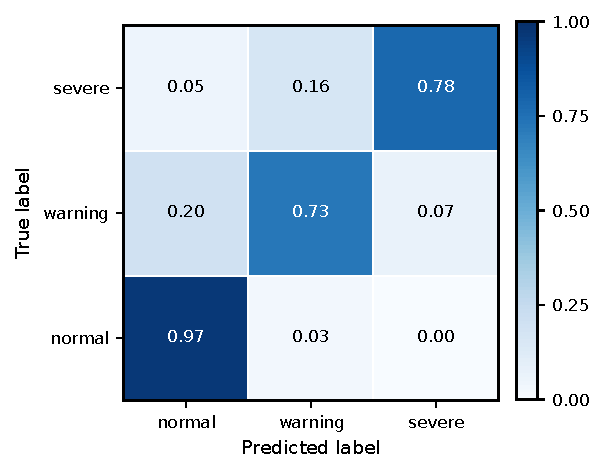
\includegraphics[width=\linewidth]{figures/confusion_matrix.pdf}
  \caption{Normalized confusion matrix, one registered \methodname{} run (TrafficCD, seed 17).}
\end{subfigure}\hfill
\begin{subfigure}{0.48\linewidth}
  \centering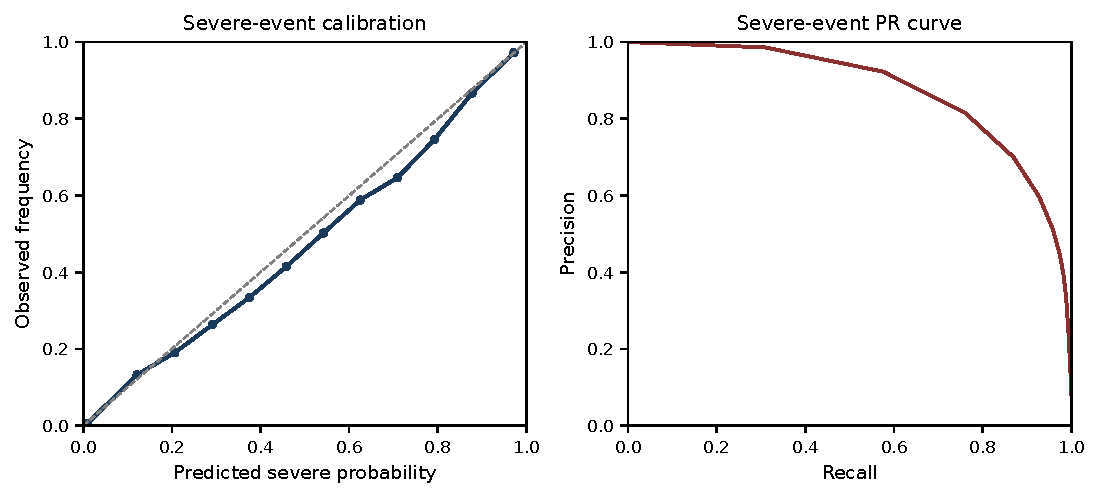
\includegraphics[width=\linewidth]{figures/calibration_pr.pdf}
  \caption{Severe-event calibration and PR curve, same run.}
\end{subfigure}
\caption{Qualitative diagnostics for one registered \methodname{} run. Source:
\texttt{outputs/studies/final\_study/main/TrafficCD/rugd/seed\_17/predictions.npz}; rendered by
\texttt{paper/figures/render\_figures.py}.}
\label{fig:qualitative}
\end{figure}

\Cref{fig:qualitative} (\Cref{sec:results-calib-eff}) gives the confusion matrix and severe-event
calibration/PR curves for one registered run (TrafficCD, seed 17). Errors concentrate between
\emph{adjacent} severity classes (normal$\to$warning: 2.95\% of true-normal examples; warning
$\to$severe and severe$\to$warning: 7.35\% and 16.47\% respectively) rather than the ordinally
distant normal$\leftrightarrow$severe confusion (0.31\% and 5.32\%), consistent with the label
space's ordinal structure even though the model is trained as an unordered 3-way classifier. We
did not curate additional qualitative failure-case examples (e.g., specific mispredicted road
segments or time windows) for this submission; the per-run \texttt{predictions.npz} files
(\texttt{time\_ids}, \texttt{node\_ids} arrays) support this directly as a follow-up.

\section{Derivations}
\label{app:derivations}

The Dirichlet-to-uniform KL divergence used in \Cref{eq:classification-loss}
(\texttt{src/traffic\_ml/losses.py::dirichlet\_kl\_to\_uniform}) is the standard closed form for
two Dirichlet distributions with concentration vectors $\boldsymbol\alpha,\boldsymbol\beta\in
\mathbb{R}_{>0}^K$:
\[
\mathrm{KL}[\mathrm{Dir}(\boldsymbol\alpha)\|\mathrm{Dir}(\boldsymbol\beta)]
= \log\frac{\Gamma(\sum_k\alpha_k)}{\Gamma(\sum_k\beta_k)} - \sum_k\log\frac{\Gamma(\alpha_k)}{\Gamma(\beta_k)}
+ \sum_k(\alpha_k-\beta_k)\big(\psi(\alpha_k)-\psi(\textstyle\sum_k\alpha_k)\big),
\]
with $\Gamma$ the gamma function and $\psi$ the digamma function; setting $\boldsymbol\beta=\mathbf 1$
recovers the uniform-Dirichlet target used throughout. \Cref{sec:analysis}'s analysis concerns
which entries of $\boldsymbol\alpha$ (equivalently $\tilde{\boldsymbol\alpha}$) are passed into this
formula, not the formula itself, which is implemented correctly against its own definition.

\section{Compute and Energy Reporting}
\label{app:compute}

Directly summing the \texttt{train\_seconds} and \texttt{inference\_seconds} columns across every
retained run gives 5{,}970s (main-suite training, 99 runs) + 5{,}693s (ablation training, 63 runs)
+ 14s + 7s (inference) $=$ 11{,}684s $\approx$ 3.25 GPU-hours for all main-suite and ablation
model-fit compute, plus 18{,}293s $\approx$ 5.08 GPU-hours for the 12 logged Optuna tuning searches
(RUGD/UIGNN/STAEformer-Inductive/OpenCity-Scratch only) --
\textbf{8.33 GPU-hours accounted for in total}, on one NVIDIA RTX 5080 (\texttt{environment.json}).
This explicitly excludes GRU/Graph-GRU's earlier, unretained tuning-pass compute (\Cref{sec:setup},
\Cref{sec:limitations}); we do not have a figure for that and do not estimate one. We did not
measure or estimate carbon emissions for this study.

\section{Reproducibility: Exact Commands}
\label{app:regenerate}

\begin{itemize}
  \item Full study from scratch: \texttt{python scripts/run\_full\_pipeline.py --study-id
        final\_reproduction --baseline-trials 30 --trials 20 --transformer-trials 8}
        (\texttt{--resume} to continue an interrupted run without repeating completed work).
  \item Verification before a long run: \texttt{python -m pytest -q} and
        \texttt{python scripts/verify\_modern\_models.py --batch-size 12 --backward}.
  \item Every number in every main-body and appendix table: \texttt{python
        paper/tables/generate\_tables.py}, reading only from
        \texttt{outputs/studies/final\_study/\{main,ablations\}/*.csv}.
  \item The headline table's bootstrap confidence intervals (\Cref{tab:headline}), using the same
        hierarchical city-then-seed bootstrap as every paired-comparison CI in this paper:
        \texttt{python paper/tables/regenerate\_headline\_ci.py}.
  \item Every figure's underlying data: \texttt{python
        paper/figures/regenerate\_figure\_data.py}.
  \item The Markdown results report this paper's numbers were cross-checked against:
        \texttt{python scripts/export\_results\_report.py} $\to$ \texttt{docs/FINAL\_RESULTS.md}.
\end{itemize}

\section{Material Relocated from the Prior Draft}
\label{app:relocated}

An earlier internal draft of this paper (never submitted; see the accompanying \texttt{
DRAFT\_TRIAGE.md} audit) contained the same core results reported here, independently re-verified
against the raw per-run CSVs during this revision (zero numeric discrepancies found). Two changes
from that draft are worth recording explicitly: (1) two subsections in that draft
("per-city ablations," "complete metric breakdown") consisted of a bare table with no interpretive
prose; the corresponding tables here (\Cref{tab:full-metrics}, and the per-city ablation numbers
folded into \Cref{app:complete-results}) are accompanied by explicit takeaways, per this paper's
own "never a table without a takeaway" standard; (2) that draft's architecture figure
(\Cref{fig:architecture}'s predecessor) was a raster illustration with decorative city-skyline
icons and no tensor-shape labels; \Cref{app:figure-redesign} documents the redesign.

\subsection{Figure redesign notes}
\label{app:figure-redesign}

The prior draft's Figure 1 used gradient-shaded blobs, decorative city-skyline icons, and
color-only encoding of block type, with no arrow-level tensor shapes and no notation tying it to
the Method section's equations. \Cref{fig:architecture} instead: (1) labels every block with the
paper's own symbols ($h_i$, $m_i$, $s_i$, $z_i$, $\alpha_i$) rather than icons; (2) annotates the
two main data-flow arrows with the fused/diffused representation symbols; (3) distinguishes
inference-path (solid) from training-only paths (dashed), a shape-redundant encoding (not
color-only) for colorblind accessibility, with the exact key given in the caption; (4) uses a
fixed, colorblind-safe palette defined locally in the figure source; (5) is pure vector TikZ with
no embedded raster content, compiling directly from \texttt{paper/figures/architecture.tex} via
\texttt{main.tex}.

This went through two internal revisions before the one in the main text. The first used
TikZ's \texttt{positioning} library (chained \texttt{right=X of Y} / \texttt{above right=X and Y
of Z} placements) rather than fixed coordinates; two independent chains that shared an anchor
node compounded their relative offsets unpredictably once rendered at full size, producing a
visible overlap between the local-evidential-head box and the diffusion block, and the legend
was built from a \texttt{matrix} of nested \texttt{\textbackslash tikz\{...\}} mini-pictures,
which is invalid outside an active \texttt{tikzpicture} context and caused a
"TeX capacity exceeded" runaway-expansion compile error. The second revision fixed both with
absolute coordinates and a legend built from plain nodes in the outer picture, but its natural
bounding box was roughly $26\times20$\,cm; scaling that down to the page width via
\texttt{\textbackslash resizebox} would have shrunk the font by the same factor as everything
else, past the point of legibility. The version in the main text compacts the coordinate grid to
roughly $19\times10.5$\,cm and moves the legend into the caption rather than drawing it in the
figure, which removes both the size problem and the class of nested-node risk that caused the
first revision's compile error, rather than only patching that one instance of it.


\end{document}
